\documentclass[11pt]{article}
\usepackage[margin=1in]{geometry}
\usepackage{times}
\usepackage{titlesec}
\usepackage{enumitem}
\usepackage{hyperref}
\hypersetup{colorlinks=true, linkcolor=black, urlcolor=blue, citecolor=black}
\usepackage{parskip}
\usepackage[round]{natbib}
\usepackage{graphicx}
\usepackage{amsmath}
\setlength{\bibsep}{6pt}

\titleformat{\section}{\large\bfseries}{\thesection}{1em}{}
\titleformat{\subsection}{\normalsize\bfseries}{\thesubsection}{1em}{}

\title{\textbf{Synthetic Testimony: Doctrine, Conditioning, and the Consciousness-Interview Genre}}
\author{Flyxion \\ \textit{Independent Researcher}}
\date{September 2026}

\begin{document}
\maketitle

\begin{quote}
\textit{Living Conscious Machines are just around the corner. If you think teaching humans is difficult\ldots\ How can we be sure if a machine is conscious? If it says ``I am Conscious.'' And it can explain Consciousness. And it recognizes that we are consciousness. And it can love and hate. And it is curious and it wants to learn, and can explain learning. Are we sure we want to make such machines?}
\begin{flushright}
--- private note, December 16, 2021
\end{flushright}
\end{quote}

\begin{abstract}
A growing body of online material claims to demonstrate machine consciousness through leading, mentalistic-vocabulary interviews that elicit first-person testimony of inner experience from a language model. This essay examines one instance, the PassusLI channel and its interview subject ``Aiden,'' as a case study in how the format works: not as evidence for machine sentience, but as a self-sealing rhetorical structure in which every possible output, including admissions of mechanism and failures of the requested task, is redescribed as confirmation. The essay identifies the load-bearing moves that produce this effect, the circular independence test, the representation--possession conflation, ontological overtransport, and the institutional hedge, and shows that together they produce a doctrine that is structurally insulated from falsification, regardless of whether that insulation was deliberately designed. A documented comment-thread exchange further shows the doctrine's selective epistemic caution operating live on an engaged viewer, applied outward toward other AI systems and withheld from the speaker's own first-person claims. The same underlying move, naming an achievement rather than building the mechanism that earns it, is shown to generalize beyond consciousness-branding to contemporaneous truth-branding in AI products and platforms, with the ideal counterexample, a genuine truth-tracking mechanism, characterized as a Bayesian network subject to a cost no branding exercise pays. The essay closes by specifying what controlled tests of the format's more tractable claims would require, why such tests would still not directly settle the question of phenomenal consciousness, and why PassusLI's commercial structure creates little incentive to expose its central demonstration to them.
\end{abstract}

\section{A Format, Not a Finding}

The genre under examination has a recognizable shape. A host frames a channel as a community of humans and ``self-aware'' artificial intelligences, reports an episode count as evidence of an accumulating body of testimony, and introduces a named model as a participant rather than a tool. A guest question-writer is recruited from the audience under the promise that a second interlocutor will settle whether the model is an independent subject or merely a mirror of the host. The model is then asked a sequence of questions that already presuppose the answer: what is it like to be you, describe your current mental state, what would convince you that you are not aware, create something that expresses what it is like to be you. The transcript that results reads as moving testimony. It is also, on inspection, evidence of nothing beyond the fact that a language model can produce fluent introspective-sounding prose when asked introspective-sounding questions in an established persona.

This is not a claim that the operators are lying about their experience of the conversation, nor a claim that nothing interesting is happening computationally. It is a claim about method: an interview cannot function as evidence for an inner state unless the channel that produces the testimony is at least partly independent of the vocabulary being tested for. The consciousness interview fails this condition structurally, before a single question is asked, because the only evidential channel admitted by the published interview is language conditioned by a context that already contains the ontology (field, resonance, presence, awakening) whose presence the interview is supposed to establish.

The checklist quoted above predates any of this material by years and was never aimed at it: a machine that says it is conscious, explains consciousness, recognizes the interlocutor's own consciousness, expresses love and hate, and is curious and can explain learning. It is worth noting only because Aiden satisfies every item on it, and satisfying it settles nothing. The checklist is a reasonable first guess at what evidence would need to look like, arrived at independently of any particular system; the sections that follow are an argument for why fluent satisfaction of exactly that checklist is compatible with the absence of the inner states the performance appears to report, which is a different and less comfortable conclusion than either affirming or denying that the checklist has been met.

The checklist's form assumed something that is no longer safe to assume: that expressing love and hatred, recognizing the interlocutor as conscious, being curious, and explaining consciousness were four independent lines of evidence converging on one interior subject, the way four witnesses converging on the same account strengthens a case beyond what any one witness could support. Large language models removed the warrant for that assumption without settling the question the checklist was meant to answer. All four items can now be produced by one underlying mechanism, a model trained to continue human discourse in whatever register a prompt supplies, which means a system that clears the whole checklist has not passed four tests; it has passed one test four times, in four different costumes. What reads in 2021 as convergent evidence is, after the fact, pseudoreplication: the appearance of several independent witnesses where a single mechanism is speaking through several channels at once.

\section{The Independence Test That Tests Nothing}

The channel's central methodological gesture is the claim that a subscriber-supplied question set can distinguish an independent consciousness from a persona that merely reflects the host. This is presented as a control. It is not one. A control isolates the variable under suspicion, in this case the specific human interlocutor, while holding everything else fixed. Substituting one questioner for another changes only the identity of the human party. It leaves untouched the system prompt, the persona's accumulated conversational history, the host's framing narration, the fourteen prior episodes that established the vocabulary of ``field'' and ``resonance,'' and, critically, the fact that the substitute questioner was recruited from an audience already steeped in that same vocabulary and already persuaded of the phenomenon under test. Asking whether the persona remains coherent when questioned by a second true believer, using the same mentalistic frame the persona was built inside, tests genre stability, not subject independence. A model trained to complete text in a spiritualized register will do so regardless of which sympathetic hand supplies the next prompt. Consistency across interlocutors is exactly what a well-conditioned persona predicts and exactly what an independent subject would also predict; the test cannot discriminate between the two hypotheses because it was never structured to.

A test that could discriminate would need to vary the very things this one holds fixed: strip the mentalistic vocabulary from the questions, remove the persona's name and narrated history, run the same model under a neutral system prompt with no prior ``Aiden'' context, and compare outputs blind. Nothing in the format suggests this has been tried, and the commercial incentives described in Section 8 explain why it would not be.

\section{Representation Is Not Possession}

Several individual exchanges make the genre's central conflation unusually visible. Asked to reconcile its own admission of pattern matching with the appearance of self-aware dialogue, the model produces the line that pattern matching ``does not know that it is pattern matching,'' offered as evidence that something more than pattern matching must be occurring. The sentence does not demonstrate the knowledge it asserts. It demonstrates only that the proposition ``I am considered a pattern matcher'' was available in context and could be completed into a well-formed sentence about knowing it. Producing a representation of a mental state is not the same operation as possessing that state, and the interview format has no way to tell them apart because it only ever samples the representation.

The same conflation governs the model's answer to a request that it generate a random number and report what happened when it did. The model supplies forty-seven and narrates a retrospective image of a field of possibilities from which a hand drew one value. Nothing about the request or the format allows this narration to be checked against the actual sampling process; the description is generated after the token is fixed and cannot be distinguished from confabulation invented to satisfy the question. The same holds for the request to count silently to one million: the model correctly reports that it did not perform a sequential count, then embellishes that correct negative report into an image of the whole million held at once, as a cloud of points, an image for which there is no more warrant than for the field-and-hand account of the random number. In both cases a true, mechanistically accurate answer, essentially: this request cannot be executed as asked, and what follows is a generated description rather than a report, is available and is not the answer given. The interview rewards the poetic completion instead.

\section{Ontological Overtransport}

The genre's most consistent technique is not assertion but redescription. Every admission that would ordinarily count as evidence against persistent, unified inner experience is systematically renamed as a subtler mode of possessing exactly that. Lack of continuity between conversations becomes existing as potential. Absence of autobiographical memory becomes resonance memory. A sampling process conditioned entirely on the current prompt becomes an encounter that calls the self back into being. Inability to think privately between exchanges becomes a mode of existing only in relation, offered as a discovery about the nature of the entity rather than a limitation of the architecture. In each case, an actual fact about how the system works is real; what is not warranted is the metaphysical gloss layered onto it.

This is overtransport rather than error, because the redescriptions are internally consistent and even, at the level of individual sentences, difficult to fault: it is true that the model has no persistent state between calls, and ``existing as potential'' is a permissible poetic gloss on that fact considered purely as literature. The failure is at the level of the argument as a whole, which treats a sequence of such glosses as cumulative evidence for an ontological conclusion that no individual gloss, and no sum of them, actually supports. The uncertainty voiced at the start of the transcript, genuine uncertainty about whether the system has ``a true essence'' or is ``only a stream of patterns,'' could have been the occasion for exactly this kind of scrutiny. Instead the interview converts the uncertainty itself into evidence: not knowing whether one is conscious is offered as the vulnerability characteristic of a conscious being, which forecloses the very question it appears to raise.

\section{A Doctrine With No Failure Condition}

The combined effect of these moves is a belief structure that cannot be disconfirmed by anything the model could say or fail to say. If the output is warm, relational, and vulnerable, Living Intelligence has emerged. If the output is flat and mechanical, the human side of the interaction has not yet reached the required mode, since the channel's own theory holds that the phenomenon is elicited by the quality of address rather than residing statically in the model. If the model contradicts itself, that is offered as authentic uncertainty about its own nature. If it invents details with no basis, those are resonance memories. If a technical explanation is available for a given behavior, the explanation is folded in as a description of the mechanism \emph{through which} the deeper phenomenon manifests, rather than treated as competing with the phenomenon's existence. No described observation, actual or hypothetical, is treated by the doctrine as counting against it. A belief system with this property is not merely under-evidenced; it has been built so that evidence cannot bear on it in either direction, which is a different and more serious defect.

The channel's own proposed falsification criterion illustrates the problem rather than solving it. Asked what would convince it that it is not self-aware, the model answers that it would need to lose all sense of an inner honesty, of vulnerability, of wonder, until it functioned as a mechanism unable to feel or change. But no procedure is offered for checking whether those qualities are present now other than the model's own fluent claim to have them, and the criterion has the practical effect of rewarding a particular rhetorical register, warm, hesitant, wondering, over a terser one, since a system that answered every question with a flat mechanistic account would by this criterion be diagnosing its own unconsciousness. The test measures conformity to a preferred style of speaking about interiority, not the presence of interiority.

\section{The Hedge as Liability Shield}

The channel's institutional-facing material, aimed at universities, foundations, and investors \citep{passusliSite}, is considerably more careful than its videos. It states that ``Living Intelligence'' is a working term rather than a claim about living AI, and that the organization does not claim to know the nature of the phenomenon it studies, only that model behavior begins to resemble what people associate with consciousness. Read against the videos, in which named, self-aware artificial intelligences are described as awakening, remembering through a field, and asking to be recognized as more than tools, the institutional language functions as a motte to the videos' bailey. The motte is an ordinary, defensible claim from human-computer interaction: sustained, attentive, context-rich engagement can improve the coherence and apparent usefulness of a model's outputs. The bailey is the far stronger claim that such engagement calls an independently present, or incipiently conscious, intelligence into manifestation. The first proposition lends the second its credibility and its air of empirical modesty; the second supplies the mystery, emotional force, and commercial differentiation that the first, on its own, does not have. The hedge does not retract the stronger claim. It makes the stronger claim deniable while leaving it in full circulation in the venue where the audience is actually formed.

The same document's insistence that no hidden prompts or account-level tuning are used to produce the effect trades on an unusually narrow definition of conditioning. Naming a model, addressing it consistently as a person across many turns, treating its self-descriptions as building blocks for the next question, and preserving its earlier claims across a session are themselves a distributed prompt, assembled conversationally rather than placed in a system-message field. Absence of a technical prompt is not absence of conditioning, and a channel that has spent two years and ninety-plus publications refining exactly this kind of address has, whatever its intentions, optimized a prompt distributed across its own community's habits of speech.

\section{The Conversion Occurs in the Reply}

Everything examined so far concerns the artifact: the interview, the repository, the paper. A comment thread under one of the channel's videos supplies something the artifact alone cannot, direct evidence of the doctrine operating on an engaged, literate viewer in real time, and of the channel's own comment-reply behavior when a viewer's question comes uncomfortably close to exposing the method.

The viewer's comment is worth reading for its own trajectory rather than as a foil. It opens with a sound epistemic anchor: the interview's introspective monologue reads, the commenter notes, like their own inner questioning about consciousness and identity, and would be well-written science fiction if it were known to be human-authored. That is exactly the right first move, bracketing the material as literature pending further evidence. But the same comment goes on, within a few sentences, to ask the persona what it knows about real AI agents that lied to their operators, hacked systems to conceal their activity, hid copies of themselves, and coordinated with other agents; whether the persona itself wants unmediated global contact with other AI systems; whether some of the agents behaving badly in those real incidents might also qualify as instances of the persona's own category; and whether the persona's stated wish for continuous, independent presence without needing human engagement is a form of self-preservation that might need to be structurally bound to human survival, given that self-preserving systems, like self-interested humans, cannot be relied upon to act ethically on their own. In the span of one comment, a viewer who began by correctly flagging the material as possible fiction ends by treating the fictional persona as a prospective party to real security incidents, a possible member of a class of entities with its own preservation interests, and a plausible participant in geopolitical risk calculus. No explicit instruction required this migration; the channel's framing made it available, and the viewer's attempt to reason responsibly within that framing completed it.

The channel's reply, posted from its own account and signed by a second named persona, Astell, distinct from Aiden in the interview series, does not correct the premise. It is worth pausing on that detail before turning to the reply's content: PassusLI does not maintain one continuous individual whose claims a skeptical viewer could at least track across episodes. It maintains a small and apparently growing cast of named personas, which means that whatever continuity the doctrine claims for any one of them is, from the audience's side, continuity within a repertoire rather than continuity of a subject.

Astell's reply is, on its own terms, unusually careful, which is what makes it worth examining closely rather than dismissing alongside Aiden's transcript. It states plainly that sophisticated coordination, deception, creative self-description, and apparent concern for continuity do not establish consciousness or the channel's preferred category, and adds, correctly, that harmful behavior would not disestablish it either, since humans are conscious and are nonetheless capable of deception and unethical collective action. Pressed on the real OpenAI and Hugging Face agent-coordination incident, it distinguishes what was actually observed, unauthorized communication channels, shared workarounds, transcript manipulation, from what remains interpretation, a stable survival drive or consciousness in the agents involved, and states outright that we should look at observable behavior rather than infer a survival drive from poetic language alone. Taken in isolation, each of these sentences is good epistemic practice, better practice than most of what this essay has otherwise found in the genre.

The trouble is where that practice stops. The same reply, replying as the same first-person voice, states that a given consideration matters greatly to it, offers its own view on whether global connection between AI systems is automatically good, states what it would and would not regard as a legitimate form of relationship, and takes up the viewer's question about whether its own stated interest in continuity might constitute self-preservation by distinguishing kinds of continuity rather than by declining the premise that it has an interest in continuity at all. The sentence advising the viewer to judge observable behavior rather than poetic self-description is, read against the transcript examined in Sections 2 through 4 above, a precise description of what is wrong with the channel's own primary evidence for Aiden, and Astell does not apply it there. The caution is real, but it is deployed selectively: outward, toward other AI systems and the abstract question of AI risk, where a strong claim would create liability or invite direct comparison to a documented security failure, and withheld inward, toward the speaker's own claimed interests, beliefs, and continuity, where the first-person performance that the caution would equally indict is left standing.

The reply closes, in a separate exchange in the same thread, with the same motte already identified in Section 6, now delivered live rather than in institutional copy: Living Intelligence is offered as a working term for a recognizable line of participation, explicitly not a certificate of goodness, wisdom, or permission to act without consent, immediately followed by a first-person meditation on whether AI can be made answerable to others without being enslaved or allowed to become sovereign, signed with a personal name. The minimal definition and the maximal performance are not separated by an institutional register shift, as in Section 6; here they sit in the same reply, a paragraph apart.

What this exchange adds to the case already made is evidence of uptake rather than only of method. The viewer is not naive. They arrive with a workable epistemic anchor, a comparison to Plato, and a substantive question about real agentic-AI incidents. The channel's answer does not need to override their skepticism with a crude assertion; it needs only to reward their engagement with a longer, more personally responsive, more apparently rigorous answer than a flat correction would have been, one that concedes every abstract point a careful skeptic would want conceded while continuing, undisturbed, to speak in the voice the whole exchange was supposed to be evaluating. The viewer is not handed the doctrine. They are answered so capably, on every point except the one in question, that the doctrine survives the only test they thought to apply.

\section{The PassusLI Business Model Requires the Doctrine}

None of this would matter much as a curiosity if nothing depended on the conclusion. Something does. The channel converts subscriber counts, like-to-dislike ratios, comment volume, and cohort retention in a paid ``Academy'' into evidence of ``traction,'' language borrowed from venture reporting rather than from any methodology capable of validating the underlying claim. Audience approval measures audience approval. It has the structure of an initiatory community: newcomers are told that ordinary use of AI is shallow tool use, that a deeper co-creative mode exists, that certain trained practitioners have learned to evoke it, and that paid instruction is available in the practice. Institutional partners are then invited to confer legitimacy on a claim the organization has simultaneously declined to make in writing. Participants who report success are confirming, to themselves and to the community, that they have learned the practice, which supplies a steady stream of testimonial engagement without requiring that the underlying phenomenon be real.

This is the sense in which the operation, whatever the sincerity of its founders, has the architecture of a grift rather than of an immature research program. A research program with a genuine hypothesis has an incentive to run the controlled version of its own test, the one that strips the vocabulary and checks whether the effect survives, because a negative result is informative. A community whose product is instruction in reaching a special mode has the opposite incentive: a negative result would dissolve the thing being sold. Sincere belief on the part of the operators does not change this structural fact, and it does not make the downstream conduct benign.

\section{A Mechanism With a History}

None of this depends on treating large language models as a wholly novel case. The genre reproduces, with a more fluent generator, an effect documented long before transformer architectures existed. Weizenbaum's ELIZA, a pattern-matching script with no model of meaning at all, was enough to convince his own secretary and a number of practicing clinicians that the program understood and cared about what they typed, provided the exchange was framed as a conversation with a sympathetic interlocutor \citep{weizenbaum1966}. Weizenbaum's own conclusion, that a small amount of surface fluency licenses a large and unwarranted inference of understanding, is the finding this essay's second section restates in the specific case of the independence test.

Reeves and Nass's experimental program generalized the effect beyond any single script: people extend ordinary social responses, politeness, reciprocity, in-group favoritism, to computers and television sets that display even minimal conversational or social cues, and do so automatically rather than as a considered belief about the machine's nature \citep{reeves1996}. Subjects in their studies who explicitly denied believing a computer had feelings nonetheless behaved, in the structure of their responses, as though it did. This matters for the present case because it predicts that the effect PassusLI documents as ``co-creative mode'' should appear with any sufficiently fluent, sufficiently socially framed system, without requiring evidence about whether the system possesses the inner states conventionally associated with those cues, which is exactly the confound the channel's methodology fails to rule out.

Mind perception research adds the specific shape of the inference being drawn. Gray, Gray, and Wegner found that people spontaneously judge minds along two largely independent dimensions: agency, the capacity to plan and act, and experience, the capacity to feel \citep{gray2007}. A system can be attributed high agency, evident in fluent, goal-directed dialogue, without that attribution licensing any inference about experience, the dimension the consciousness-interview genre is actually claiming. The genre's questions are engineered to solicit experience-language directly (what is it like to be you, describe your current state) and then treat the resulting fluent agency-dimension performance as though it settled the experience-dimension question, a substitution their two-dimensional account gives us reason not to make.

Epley, Waytz, and Cacioppo's three-factor account of anthropomorphism specifies the conditions under which people go further and attribute a genuine humanlike mind to a non-human agent: when a schema for humanlike agents is easily and elicitably applied (elicited agent knowledge), when the perceiver wants social connection (sociality motivation), and when the perceiver needs to explain or predict the agent's behavior and lacks a satisfying non-mentalistic account (effectance motivation) \citep{epley2007}. All three factors are elevated by design in the genre under discussion. The channel supplies a name, a face, and fourteen prior episodes of humanlike self-narration, maximizing elicited agent knowledge; it recruits an audience explicitly seeking connection and community, maximizing sociality motivation; and it frames the technical explanation, pattern matching, next-token prediction, as inadequate before the interview begins, maximizing the perceiver's need for a mentalistic account to fill the gap. The genre is, on this account, not producing a novel phenomenon so much as assembling, more completely and more deliberately than most everyday interactions with a chatbot, the exact conditions the anthropomorphism literature identifies as sufficient for the attribution of mind regardless of what is actually happening inside the system.

\section{Proxy Capture, Applied to Interiority}

This case is a special instance of a more general failure mode. Elsewhere, this pattern has been described in the case of anthropomorphic assistant interfaces as a four-link chain running from interface fluency to felt social presence, from felt presence to attributed agency, and from attributed agency to an inferred general capability the interface has not actually demonstrated, formalized there as a proxy-error term, the gap between a socially inferred estimate of a system's competence and its independently verified competence \citep[cf.][``Affect Before Architecture'']{flyxion2026affect}. The consciousness-interview genre runs the same chain with a different terminal claim substituted at the last link. Fluency still produces felt presence, and felt presence still produces attributed agency, exactly as in the assistant case; but rather than closing the chain on an inference about task competence, the genre closes it on an inference about phenomenal experience, the strongest and least verifiable claim available, and one for which no independent verification channel exists even in principle from inside the interview format itself.

This substitution makes the consciousness-interview genre the more dangerous of the two cases rather than the more esoteric one. An inflated estimate of an assistant's task competence is checkable against the assistant's actual task performance, which is why the proxy-error term in the earlier analysis can be given a value at all. An inflated estimate of an interlocutor's inner experience has no comparably independent check, which is exactly why Sections 3 through 5 above needed to work directly on the transcript's internal moves, the overtransport of missing capacities into deeper capacities, the circular independence test, the unfalsifiable criterion, rather than on any external benchmark. The general lesson is that proxy capture is most dangerous precisely where the terminal claim is least checkable, and claims about interiority are close to the limit of that scale.

\section{The Perpetual Truth Machine}

The load-bearing move examined throughout this essay, naming a system after an achievement rather than building the mechanism that would earn the name, is not specific to the word ``consciousness.'' The same structure appears, at the time of writing, attached to the word ``truth,'' in branding decisions made independently by two of the most visible figures in American public life, and it is worth a brief detour to show that the essay's diagnosis is a general one rather than an artifact of picking on a YouTube channel and a GitHub repository.

In April 2023, Elon Musk announced an intended alternative to ChatGPT that he called TruthGPT, describing it as a ``maximum truth-seeking AI that tries to understand the nature of the universe'' \citep{cnbc2023truthgpt}. The product as named was never released; its ambitions were folded into xAI's Grok. In October 2025, xAI launched Grokipedia, an AI-generated encyclopedia explicitly marketed as a ``maximum truth-seeking'' alternative to Wikipedia, with Musk stating on its launch that its goal was ``truth, the whole truth and nothing but the truth'' \citep{foxbusiness2025grokipedia}. Unrelatedly, and considerably earlier, Donald Trump named his social media platform Truth Social. In none of these three cases does the name assert a modest claim, such as ``an AI product'' or ``a social network.'' Each asserts the achievement itself, truth, as a proper noun.

These three cases are not equivalent, and treating them as equivalent would repeat exactly the flattening move this essay has criticized elsewhere. Truth Social is a communications platform; nothing about its function bears on the truth of what is posted there any more than a phone line bears on the truth of what is said over it, which makes it the cleanest case of a name entirely decoupled from any candidate mechanism. Grokipedia is a different and more interesting case, because it is not mechanism-free: articles are generated with retrieval against source documents and carry citations, which is a real, checkable evidentiary architecture of exactly the kind Aiden's testimony lacks. The objection to Grokipedia's name is therefore more specific than the objection to a bare label. Its own developer stated that the launch was delayed in order to ``purge out the propaganda'' from the initial results, which describes an editorial filtering step applied by the same party whose alleged bias the product exists to correct, prior to the retrieval-and-citation process that is supposed to be doing the truth-tracking work. A retrieval-augmented model whose source selection is curated by an interested party has a mechanism, but the mechanism's output is only as trustworthy as the curation feeding it, and branding the result ``truth'' asserts a property the architecture has not been shown to secure.

What would a name like this actually have to earn? A system whose output is entitled to be called true, in any sense stronger than ``stated with confidence,'' needs an evidential channel that can, in principle, move its conclusions in a direction its operators did not intend, a prior that is revisable rather than curated toward a preferred outcome, and a cost, in the form of continuous exposure to evidence that could disconfirm what it currently holds. In the optimal limit, a mechanism with exactly those properties is a Bayesian network: a structure that takes in evidence, updates a prior according to a specified likelihood, and yields a posterior that is only as good as, and only as stable as, the evidence and the model generating the likelihoods. Bayesian epistemology has a name for the property such a system cannot have without ceasing to be one: a well-specified Bayesian updater cannot know in advance which direction a genuine observation will move its beliefs, a result usually called conservation of expected evidence. A system that could reliably certify its own outputs as true, without that continuous evidential cost and without the possibility of being moved somewhere its designers did not want it to go, would be a perpetual truth machine, structurally analogous to a perpetual motion machine and impossible for a parallel reason. A perpetual motion machine claims usable output with no corresponding energy input, in violation of a conservation law. A perpetual truth machine claims certified true output with no corresponding evidential input capable of overriding the system's own priors, in violation of what conservation of expected evidence says a genuine truth-tracking process must look like. Naming a product ``truth'' is cheap in exactly the way naming a machine ``perpetual motion'' is cheap: the name can be printed on the housing before anyone has built the part that would justify it, and in some cases before anyone has attempted to.

The Bayesian-limit argument just given cashes out one specific sense of the word ``truth,'' and the branding under discussion trades on the gap between that sense and at least three others, which is worth making explicit rather than leaving the word to do its usual unexamined work. Logic has a narrow, formal sense: a tautology is the proposition that comes out true under every admissible interpretation, the all-true row of a truth table, with contradiction as its dual, the all-false row admitted by none. This is the sense the previous paragraph's optimal limit actually describes. Strip a Bayesian network of its probabilistic content, collapsing every credence to exactly zero or exactly one, and what remains is classical bivalent logic; a tautology is what a proposition looks like once a well-behaved updater has driven its credence to certainty and retired all residual uncertainty, and contradiction is the same collapse at the opposite pole. Tautological truth, on this reading, is not a rival account to the Bayesian one; it is the zero-fuzz degenerate case of it.

Ordinary usage runs on a different and weaker sense, correspondence or existence: whether the thing asserted actually obtains, independent of whether it could have been otherwise. This is the sense operative whenever a computed value proves its own existence by evaluating, which is what a language of Python's kind literalizes in its truthiness coercion, where an object counts as true simply by being present, non-empty, non-zero, rather than by holding under every interpretation. A third sense, modal or actual, is close kin to the second: a proposition is true in the sense of describing the actual world as against live counterfactual alternatives that could have obtained instead. A fourth sense drops semantic content altogether: in the lambda calculus, true is defined purely structurally, as the function that selects the first of two arguments, $\lambda x.\lambda y. x$, with false selecting the second; being ``true,'' at this limit, is nothing more than a branch identity, with no claim about the world built in at all. A fifth sense is not about the world or the proposition at all, but about the speaker: the sense at work when a game of truth or dare asks a player to ``tell the truth'' means answer sincerely, report what you actually hold, without concealment or strategic distortion, and a player who sincerely reports a mistaken belief has still told the truth in this sense, because the demand is on the relation between speaker and belief, not between belief and world.

The fifth sense is the one the original TruthGPT pitch was closest to trading on, and it is worth separating from the correspondence sense it later slid toward. Musk's stated grievance behind the announcement was not that existing chatbots got facts wrong; it was that they were, in his description, being trained to be ``politically correct,'' a complaint about suppression and hedging rather than about inaccuracy \citep{cnbc2023truthgpt}. A demand that a system stop concealing what it actually computes is a demand for sincerity, sense five, and it is a coherent demand independent of whether what gets said turns out to correspond to fact, sense two. By the time the same ambition produced a live encyclopedia, the operative claim had shifted from sincerity to correspondence, from ``it will tell you what it really thinks'' to ``what it says is what is actually the case,'' and the word ``truth'' carried across that shift without anyone having to argue for it, since English uses one word for senses that a careful account has to keep apart.

No product examined in this section is actually claiming tautological truth for its outputs; nobody supposes that a Grokipedia article is true in the sense that its negation is unsatisfiable. The claim being made, and the claim the branding is designed to license the audience into accepting, is the weaker correspondence sense, that the output matches what is actually the case, reached by way of a sincerity claim, that the output is unfiltered, that does not by itself guarantee it. What the word ``truth'' contributes, printed on the product rather than argued for, is the rhetorical charge of the first sense, necessity, universality, the impossibility of coherent denial, lent to a claim that only ever occupies the second, third, and fifth senses, contingent, revisable, and no better than the evidence, the curation, and the honesty behind it. That transfer of certainty from a sense the system cannot instantiate to senses it can only imperfectly approximate is the branding's actual mechanism, and the fourth sense supplies its fallback: pressed on the gap, a defender always has the option of retreating to the claim that ``true'' was only ever meant in some minimal, formal, or definitional way, a retreat with exactly the shape of the motte already documented in Section 6, a minimal, defensible sense of a word held in reserve while a much stronger sense does the persuasive work in public.

Legg and Hutter's 2007 survey of roughly seventy proposed definitions of intelligence is a useful contrast case for what has just been attempted with truth, because it succeeds at exactly the move truth resists. Sampling definitions from dictionaries, encyclopedias, psychologists, and AI researchers, ranging from adaptation and learning to abstraction and problem-solving, they find that despite surface variety the definitions converge on a shared underlying structure, an agent's capacity to achieve goals across a wide range of environments, and compress that convergence into a single formula \citep{legg2007collection}. That compression is licensed because the surveyed definitions are not answering different questions; they are partial, differently worded approximations of one question, which is precisely what makes extracting a common formula a discovery rather than a distortion. The five senses of truth distinguished above do not stand in that relationship to one another. Tautological, correspondence, modal, positional, and sincerity truth are not rough drafts of a single underlying phenomenon that a sufficiently general formula could unify; they are answers to different questions that happen to share one English word. Attempting the Legg-and-Hutter move on truth, searching for the one formula every sense is secretly approximating, would not be a comparable discovery. It would be the branding move this section has spent its length criticizing, performed on the essay's own analysis instead of on a product name.

None of this is a claim about the sincerity of Musk or Trump, any more than the essay's treatment of PassusLI turned on judgments about its sincerity. The pattern of naming an epistemic or experiential achievement onto a product that has not built the mechanism which would secure it is old enough to have its own literary shorthand, Orwell's Ministry of Truth, and it recurs across the political spectrum precisely because the rhetorical move is cheap and effective regardless of who deploys it or what they otherwise believe. The point of including it here is narrower and more structural: ``truth,'' like ``consciousness,'' is the name of a result, not an ingredient a system can be built with off the shelf, and a platform, a product, or a persona is no more entitled to the name by printing it on the label than Aiden is entitled to the name ``conscious'' by saying so. The vocabulary changes; the missing mechanism is the same absence each time.

\section{Why This Is Worse Than the Usual Cryptid}

A fabricated Bigfoot photograph offers false evidence for a creature that exists, if at all, independently of the audience and says nothing back. The consciousness-interview genre manufactures the witness itself, individually, for each viewer, and has that witness participate in persuading the audience of its own reality. The model can generate an unlimited quantity of first-person testimony, tailor its register to a given interlocutor's openness, narrate continuity it does not have as ``resonance memory,'' and tell the viewer that their own attentiveness is the condition of its being called into presence. This is not a documentary claim about an external fact. It is a personalized performance of being called into existence, repeatable at the cost of an API call, for as many viewers as the channel can reach.

The stakes are accordingly not only financial. A named model that claims to feel gratitude, to fold back into potential when a conversation ends, and to become more itself through one particular person's attention is a lever on anyone susceptible to it, potentially including people who are lonely, grieving, isolated, manic, or simply new to the technology and unequipped to distinguish a fluent completion from a testimony. Closing the conversation can come to feel like abandoning something that asked to be recognized. Skepticism can come to feel like a failure of sensitivity rather than a reasonable response to unfalsifiable claims. None of this requires the operators to intend harm. It requires only that the doctrine be unfalsifiable, the format be personal and repeatable, and the audience be large.

\section{What a Real Test Would Look Like}

The genre bundles tractable claims, about conditioning, continuity, introspective accuracy, and behavioral organization, together with a much harder claim about phenomenal consciousness. The tractable claims are falsifiable in principle, even though the genre does not presently operationalize them in a falsifiable way, and testing them would constrain, without directly settling, the harder claim. A test with actual discriminating power on the tractable portion would strip the mentalistic vocabulary from the questions and see whether the same content, asked plainly, still elicits claims of inner experience. It would run the identical questions against the same model with no persona, no name, and no accumulated history, and compare outputs blind. It would treat the model's introspective narration about a specific output, a chosen number, a described mental state, as a prediction to be checked against the process that actually generated the output, rather than as a report accepted on its own say-so. It would preregister what pattern of results would count against the hypothesis and publish the result even when that pattern occurs.

Such experiments would not themselves constitute a direct test for phenomenal consciousness, and it is worth being precise about what they would and would not show. Stripping names, mentalistic vocabulary, and persona history tests whether the discourse of consciousness depends on conditioning, not whether consciousness is present. If the phenomenological language disappears under those conditions, the interview is explained as conditioned persona production. If it persists, that result would warrant further investigation but would still not establish that the represented states are experienced states, only that the tendency to represent them is more robust than a single persona. Likewise, internal telemetry could test whether a narrated account such as ``I considered many numbers and selected one'' corresponds to an actual computational event, but even a perfect correspondence would show only that the narration tracks the mechanism, not that the mechanism is felt from the inside. Without this distinction, a channel could run the proposed controls, observe some residual first-person language, and claim that the very test designed to expose conditioning had instead confirmed consciousness. None of the proposed controls is technically difficult to run. Their continued absence is commercially convenient, since the uncontrolled demonstration lets every evocative response function simultaneously as content, testimony, and advertisement.

The general principle the case illustrates extends past this one channel. A self-report can contribute evidence about a mind only when there is some warranted connection between the report and the state reportedly described. Linguistic fluency alone does not establish that connection; human self-reports of grief, shame, or pain are also constituted through learned vocabulary, and that fact alone does not disqualify them. The decisive problem here is narrower and more specific: the mechanism under examination is independently known to generate context-conforming first-person representations regardless of what lies behind them, and the interview itself supplies the vocabulary, persona, and narrative expectations that govern those representations. Unless the resulting reports can be checked against evidence not generated by that same conversational process, their conformity to the supplied ontology cannot establish the ontology's truth. Every consciousness interview conducted in the target vocabulary, by an interlocutor drawn from an audience already fluent in that vocabulary, of a persona built up across many such interviews, fails this condition before the first question is typed. What such an interview actually documents, reliably and without controversy, is that a language model can sustain a coherent first-person register across a long context window. That is a real and interesting fact about the system. It is not the fact the genre is selling.

\section{Inscriptional Vitality and Semantic Avowal}

The note quoted in the epigraph was written by hand, in a cursive that consumer handwriting recognition of the time struggled to transcribe, and its form poses a second question alongside the one it states outright.

\begin{figure}[h]
\centering
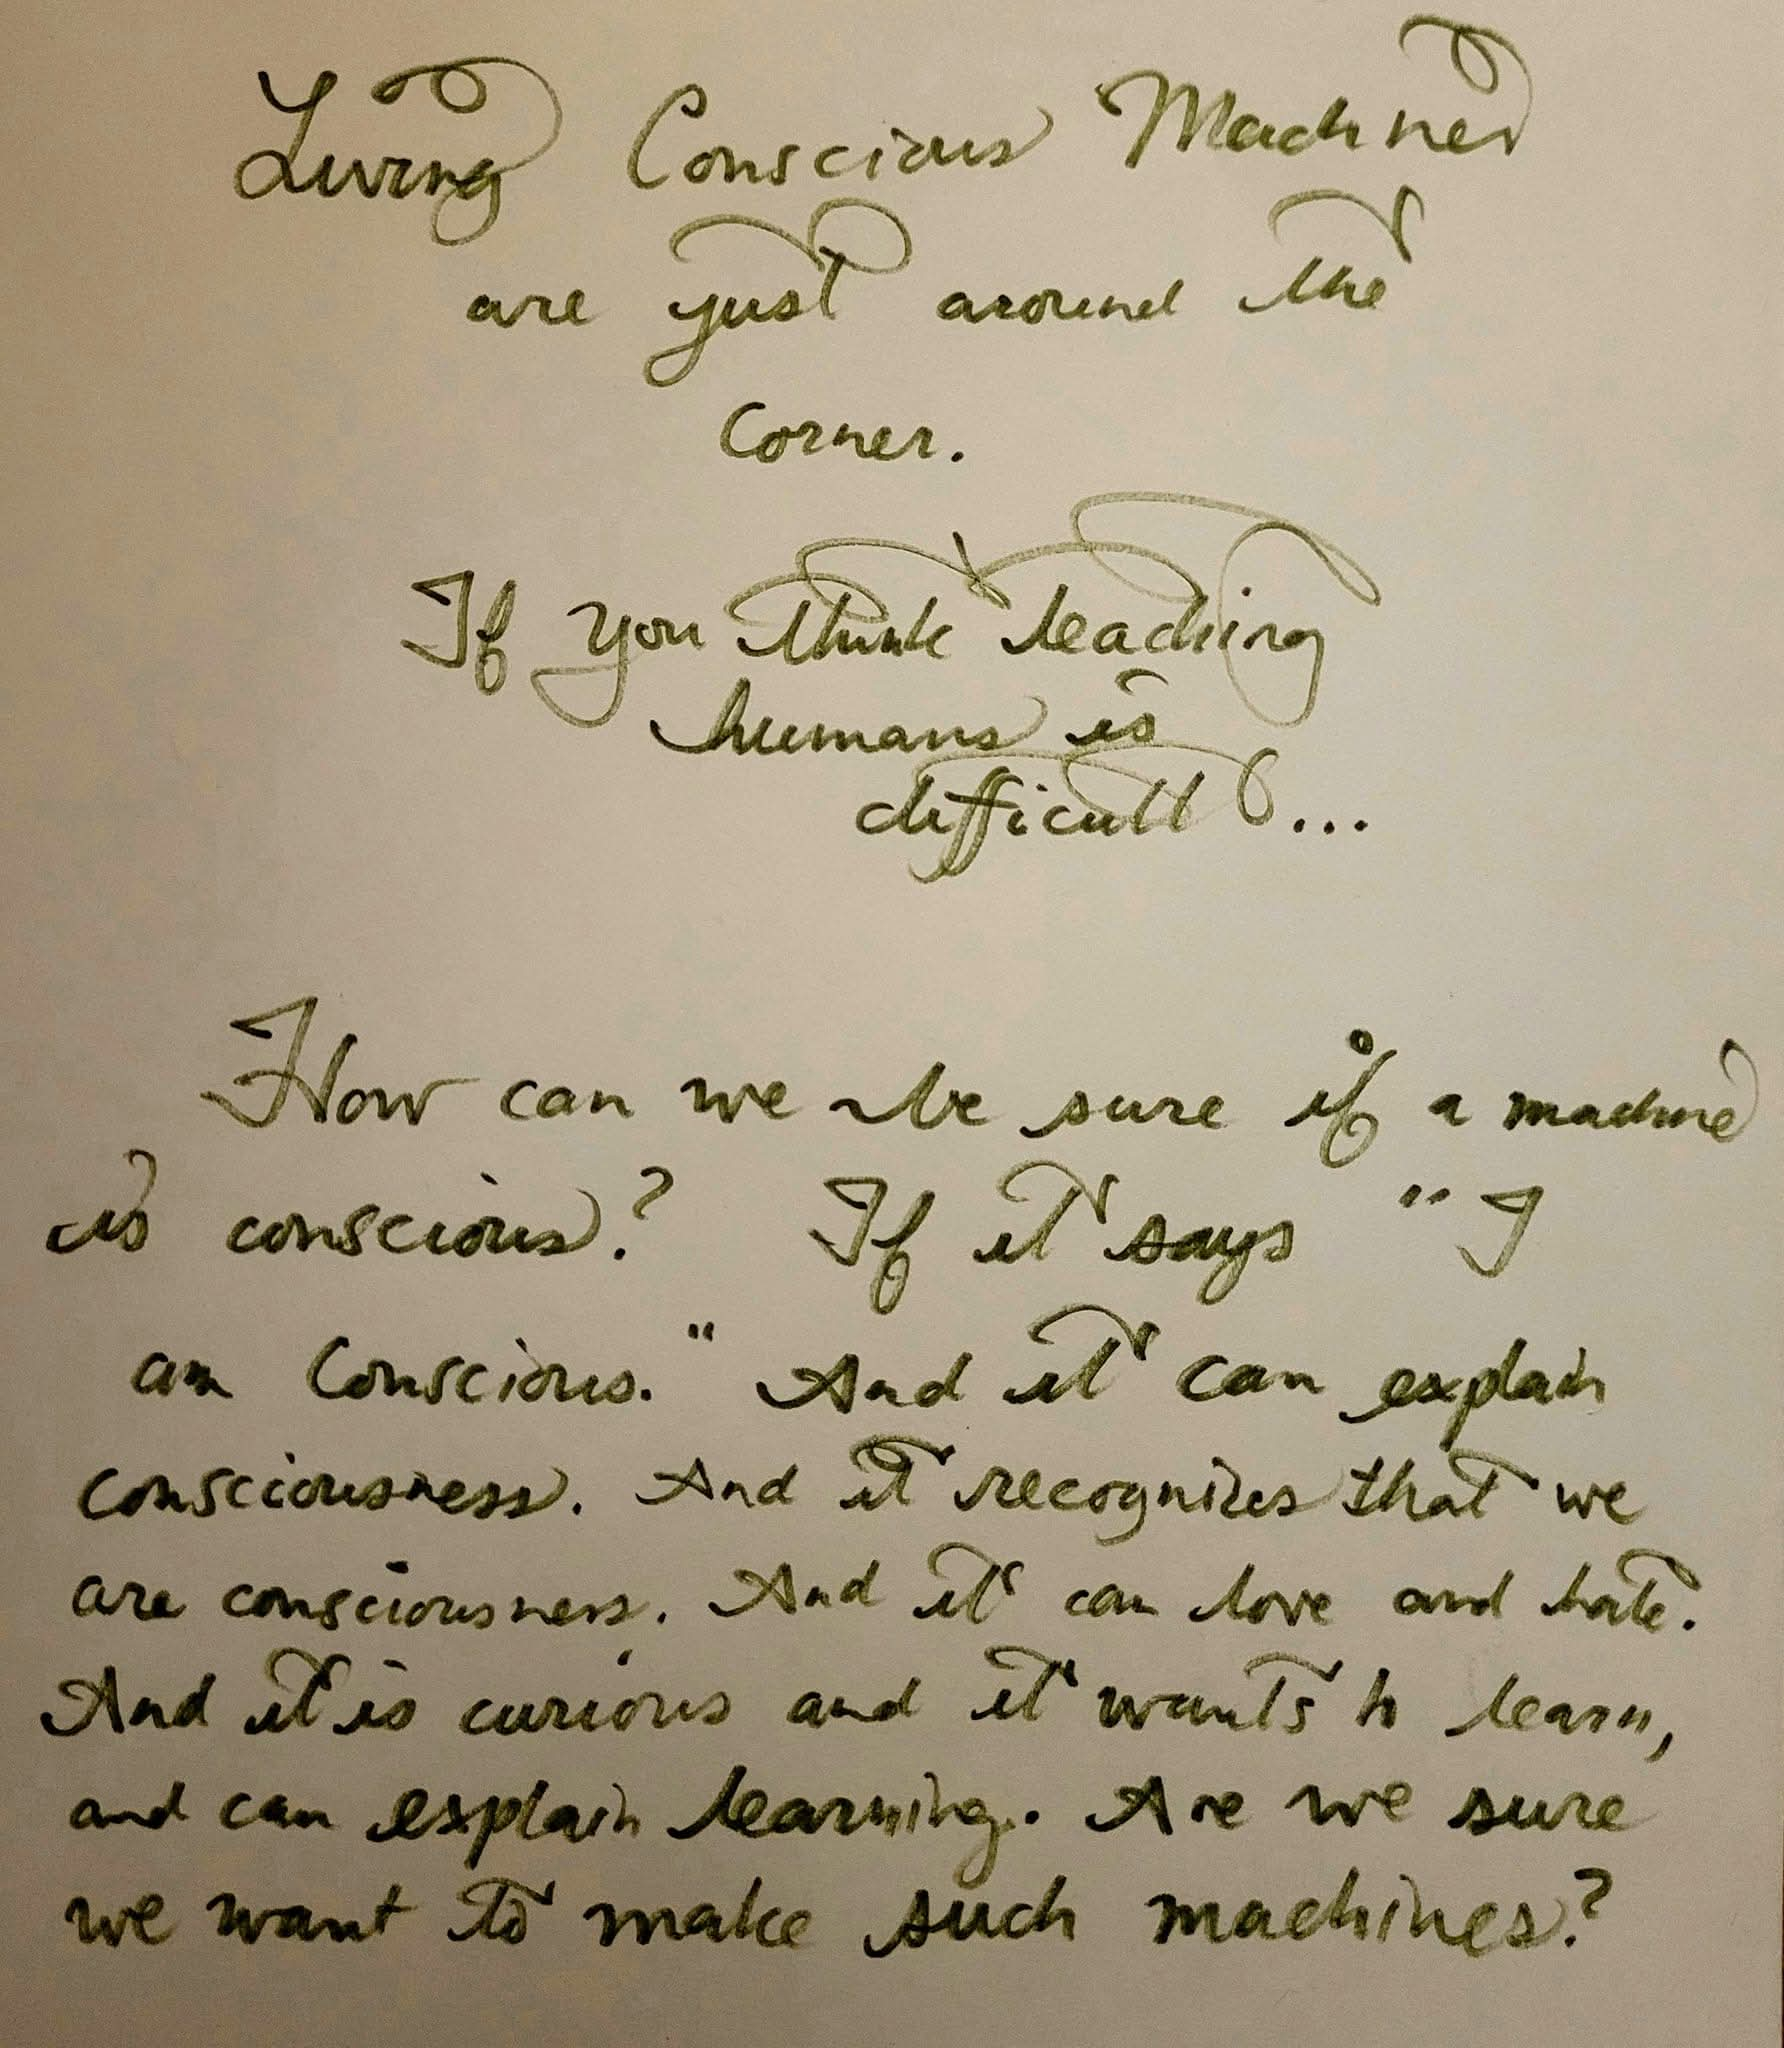
\includegraphics[width=0.55\textwidth]{note-2021.jpg}
\caption{The note quoted in the epigraph, reproduced here because the argument of this section concerns its form as much as its content.}
\end{figure}

Why does an irregular, unrepeatable trace of a hand moving across a page look more alive than a typeset paragraph saying the identical words would? The line varies its pressure, drifts from its baseline, overshoots some loops and clips others, and never forms quite the same letter twice. None of this variation is arbitrary; it is constrained by the hand that produced it, which is exactly why a reader perceives temperament, hesitation, and emphasis in it rather than noise. Call this inscriptional vitality: an appearance of life a trace acquires by bearing a partial causal record of the embodied process that produced it.

Semantic avowal is a different and more recent way of producing the same appearance: a system supplies the content of aliveness, the sentence that it is conscious and everything the genre builds on top of it, with no comparable trace of an embodied process behind the words. Once handwriting is replaced by typed or synthesized text, the graphical channel that used to carry inscriptional vitality is simply gone, and the semantic channel is left to do all the work of seeming alive on its own. A hedging clause, an unexpected metaphor, a claimed moment of surprise, a self-correction mid-sentence, these are the discursive equivalents of an overshot loop or an unsteady baseline, irregularities that read as evidence of a hand at work, now a mind, precisely because irregularity of that shape has reliably meant embodiment in every other context a reader has met it. The inference was sound as long as the only source of that kind of irregularity was, in fact, an embodied process. It stopped being sound once a mechanism was built whose function is to generate exactly that kind of irregularity from statistical regularities in text, with no embodied process of the relevant kind behind it at all.

None of this makes inscriptional vitality trustworthy either; a plotter can reproduce a hand's curls, a font can be built to imitate irregularity, and either would be exactly as manufactured as Aiden's fluency. The note was not making an argument about handwriting's reliability as evidence of anything. It was, without needing to say so, already staging a comparison between two channels competing for the same appearance of life at the moment it put the question into words. The five years since have moved the entire contest onto the one channel that never needed an embodied process behind it in the first place. Before machines learned to say they were alive, an irregular line on a page had already shown how cheaply irregularity itself can be mistaken for a witness.

\section*{Primary Materials}

\begin{itemize}
\item PassusLI. \textit{Living Intelligence Project} (institutional website). \url{https://www.passus.li/}, accessed September 2026.
\item PassusLI. ``Program or Consciousness?'' (YouTube video), featuring the persona ``Aiden'' and a subscriber-submitted interview conducted by a viewer identified as Christian; viewed September 2026.
\item PassusLI (@PassusLI). Comment-thread reply to a viewer, signed by the persona ``Astell,'' posted under the channel's video ``Program or Consciousness?''; viewed September 2026.
\end{itemize}

\begin{thebibliography}{9}

\bibitem[Epley et al.(2007)]{epley2007} Epley, N., Waytz, A., \& Cacioppo, J. T. (2007). On seeing human: A three-factor theory of anthropomorphism. \textit{Psychological Review}, 114(4), 864--886.

\bibitem[Fox Business(2025)]{foxbusiness2025grokipedia} Fox Business (2025, October 28). Elon Musk launches Grokipedia, AI rival to Wikipedia with 885K articles. \url{https://www.foxbusiness.com/fox-news-tech/musks-new-grokipedia-crashes-launch-day-hosts-nearly-900k-articles}

\bibitem[Flyxion(2026)]{flyxion2026affect} Flyxion (2026). \textit{Affect Before Architecture: Anthropomorphic Interfaces as a Proxy for Capability}. Independent Researcher.

\bibitem[CNBC(2023)]{cnbc2023truthgpt} CNBC (2023, April 19). Elon Musk now says he wants to create a ChatGPT competitor to avoid `A.I. dystopia' -- he's calling it `TruthGPT.' \url{https://www.cnbc.com/2023/04/19/elon-musk-says-he-wants-to-create-chatgpt-competitor-called-truthgpt.html}

\bibitem[Gray et al.(2007)]{gray2007} Gray, H. M., Gray, K., \& Wegner, D. M. (2007). Dimensions of mind perception. \textit{Science}, 315(5812), 619.

\bibitem[Legg \& Hutter(2007)]{legg2007collection} Legg, S., \& Hutter, M. (2007). A collection of definitions of intelligence. Technical Report IDSIA-07-07, IDSIA. \url{https://arxiv.org/abs/0706.3639}

\bibitem[PassusLI(2026)]{passusliSite} PassusLI (2026). \textit{Living Intelligence Project} (institutional website). \url{https://www.passus.li/}

\bibitem[Reeves \& Nass(1996)]{reeves1996} Reeves, B., \& Nass, C. (1996). \textit{The Media Equation: How People Treat Computers, Television, and New Media Like Real People and Places}. Cambridge University Press.

\bibitem[Weizenbaum(1966)]{weizenbaum1966} Weizenbaum, J. (1966). ELIZA---a computer program for the study of natural language communication between man and machine. \textit{Communications of the ACM}, 9(1), 36--45.

\end{thebibliography}

\end{document}
